\documentclass[12pt]{article}
\usepackage{fullpage,enumitem,amsmath,amssymb,graphicx,grffile,float,listings}



\begin{document}
    %Title Section
    \begin{flushleft}
    \LARGE CS229 Fall 2017\\
    \LARGE Problem Set \#1: Supervised Learning\\
    \textbf{\normalsize Author: LFhase \quad rimemosa@163.com}
    \end{flushleft} 
    \noindent
    \rule{\linewidth}{0.4pt}
    %Title Section

    %Problem and Solution

    \section*{Logistic regression  }

    \begin{enumerate}[label=(\alph*)]

    \item 
    {
        Given that 
        $$J(\theta)= \frac{1}{m} \sum_{i=1}^{m}log(1+e^{-y^{(i)}\theta^{T}x^{(i)}})$$\\
        we can get
        $$\frac{\partial J(\theta)}{\partial \theta_{i}}
            =  \frac{1}{m} \sum_{k=1}^{m} \frac{-y^{(k)}x^{(k)}_i}{1+e^{y^{(k)}\theta^{T}x^{(k)}}}
        $$\\
        then
        $$\frac{\partial J(\theta)}{\partial \theta_{i} \partial \theta_{j}}
            =  \frac{1}{m} \sum_{k=1}^{m} 
            \frac{x^{(k)}_ix^{(k)}_je^{y^{(k)}\theta^{T}x^{(k)}}}
            {(1+e^{y^{(k)}\theta^{T}x^{(k)}})^2}
        $$\\
        which is $ H_{ij} $\\
        so
        \begin{equation*} 
        \begin{split}
            Z^THZ &= \sum_{i=1}^n \sum_{j=1}^n z_iH_{ij}z_j \\
            &= \frac{1}{m} \sum_{k=1}^{m} 
            \frac{\sum_{i=1}^n \sum_{j=1}^n z_ix^{(k)}_ix^{(k)}_jz_je^{y^{(k)}\theta^{T}x^{(k)}}}{(1+e^{y^{(k)}\theta^{T}x^{(k)}})^2}
            \\
        \end{split}
        \end{equation*} 
        known that 
        $$ \sum_{i=1}^n \sum_{j=1}^n z_ix^{(k)}_ix^{(k)}_jz_j = (X^TZ)^2 \geq 0 $$
        $$ \frac{e^{y^{(k)}\theta^{T}x^{(k)}}}{(1+e^{y^{(k)}\theta^{T}x^{(k)}})^2} > 0 $$
        we can easily get $$ Z^THZ \geq 0 $$
    }
    \newpage
    \item 
    {
        Firstly, we plot the original data

        \begin{figure}[H]
            \centering
            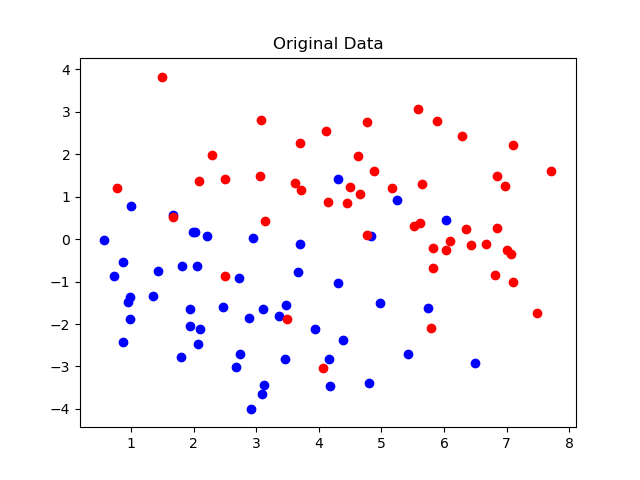
\includegraphics[width=0.80\textwidth]{figure/LogisticRegression/original_data.png}
        \end{figure}

        To implement Newton’s Method, we calculate the value of 
        $$\frac{1}{m} \sum_{k=1}^{m} \frac{-y^{(k)}x^{(k)}_i}{1+e^{y^{(k)}\theta^{T}x^{(k)}}}
        $$
        and $\textbf{Hessian}$\\
        then using the \textbf{update rule}
        $$ \theta := \theta - H^{-1}\bigtriangledown_\theta l(\theta) $$
    }
    
    \newpage
    \item 
    {
        Through 6 iterations, we finally get the result
        \begin{figure}[H]
            \centering
            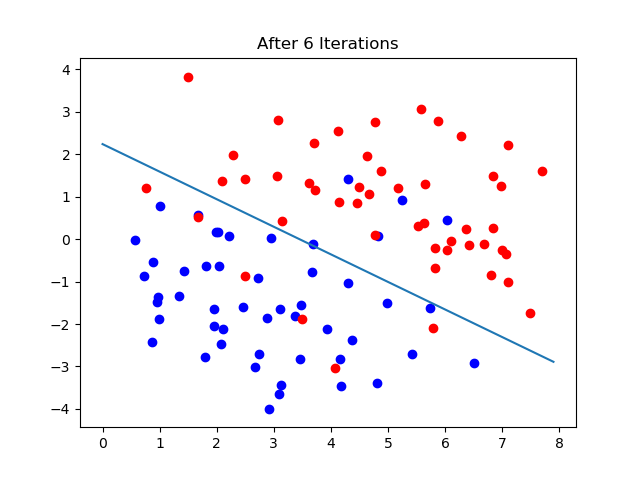
\includegraphics[width=0.80\textwidth]{figure/LogisticRegression/Iteration6.png}
        \end{figure}
        and the $ \theta $ is  [-2.6205116,   0.76037154,  1.17194674].
    }

    \end{enumerate}

    \newpage
    \section*{ Poisson regression and the exponential family}

    \begin{enumerate}[label=(\alph*)]

    \item 
    Firstly, we get 
    \begin{equation*} 
        \begin{split}
            p(y;\lambda) &= \frac{e^{-\lambda}\lambda^{y}}{y!} \\
            &= \frac{1}{y!}exp(log\lambda^y - loge^\lambda) \\
            &= \frac{1}{y!}exp(log\lambda y - \lambda) \\
    \end{split}
    \end{equation*} 
    It's easy to know that
    $$ log\lambda = \eta, \lambda = e^\eta $$
    $$ T(y) = y $$
    $$ a(\eta) = -e^\eta $$
    $$ b(y) = \frac{1}{y!} $$
    and Poisson distribution is in the exponential family.

    \item 
    Known that if $ Y \sim P(\lambda) $, then $ E[Y] = \lambda $ ,
    \begin{equation*} 
        \begin{split}
            h_\theta(x) &= E[y|x;\theta] \\
                        &= \lambda \\
                        &= e^\eta = e^{\theta^Tx} \\
        \end{split}
    \end{equation*} 
    so the response function for the family is 
    $$ g(\eta) = e^\eta $$.

    \item 
    Firstly, we can get likelihood function $L(\theta)$
    \begin{equation*} 
        \begin{split}
            L(\theta) &= \Pi_{k=1}^m P(y^{(k)}|x^{(k)};\lambda) \\
                      &= \Pi_{k=1}^m \frac{e^{-\lambda}\lambda^{y^{(k)}}}{y^{(k)}!} \\
        \end{split}
    \end{equation*} 
    Then, the log-likelihood function $l(\theta)$
    \begin{equation*} 
        \begin{split}
            l(\theta) 
            &= \sum_{k=1}^m (-logy^{(k)}!) + (-\lambda) + y^{(k)}log\lambda \\
            &= \sum_{k=1}^m (-logy^{(k)}!) + (-e^{\theta^Tx^{(k)}}) + y^{(k)}\theta^Tx^{(k)} \\
        \end{split}
    \end{equation*} 

    Then, we can get the derivative of the log-likelihood with respect to $\theta_i$
    $$ \frac{\partial l(\theta)}{\partial \theta_i} 
       = \sum_{k=1}^m (y^{(k)}-e^{\theta^Tx^{(k)}})x^{(k)}_i
    $$
    So, the stochastic gradient ascent learning rule is
    $$ \theta_i = \theta_i + \alpha(y^{(k)}-e^{\theta^Tx^{(k)}})x^{(k)}_i
    $$

    \item 
    
    Firstly, we can know that
    $$ p(y|x;\theta) = b(y)exp(\eta^Ty-a(\eta)) $$
    then, for a simple training data $(x,y)$ in stochastic gradient ascent,
    $$ \frac{\partial p(y|x;\theta)}{\partial \theta_i} 
        = x_i(y-\frac{\partial a(\eta)}{\partial \eta})
    $$
    known that,
    $$ \int_{y}p(y|x;\eta) = 1 $$
    we can imply derivation in both sides, and get
    $$ \int_{y}p(y|x;\eta)(y-\frac{\partial a(\eta)}{\partial \eta}) = 0 $$
    finally, we get
    $$ \frac{\partial a(\eta)}{\partial \eta} = \int_{y}p(y|x;\eta)y = h_\theta(x) $$
    so the gradient we get is
    $$ \frac{\partial p(y|x;\theta)}{\partial \theta_i} 
        = x_i(y-h_\theta(x))
    $$
    the update rule is
    $$ \theta_i = \theta_i - \alpha(h_\theta(x)-y)x_i $$
    \end{enumerate}

    

    \newpage
    \section*{Gaussian discriminant analysis   }
    \begin{enumerate}[label=(\alph*)]
    
    \item 
    Firstly, we have
    \begin{equation*} 
        \begin{split}
            p(y=1|x;\phi, \Sigma, \mu_1, \mu_-1)
             &= \frac{p(x|y=1)p(y=1)}{p(x|y=1)p(y=1)+p(x|y=-1)p(y=-1)}  \\
             &= \frac{1}{1+\frac{p(x|y=-1)p(y=-1)}{p(x|y=1)p(y=1)}} \\
        \end{split}
    \end{equation*}                                                                                                                                                                                                                                                                                                                                                                                                                                                                                                                                                                                                                                                                                                                                                                                                                                                                                                                                                                                                                                                                                                                                                                                                                                                                                                                                                                                                                                                                                                                                                                                                                                                                                                                                   
    apply such calculattion, we can get
    \begin{equation*} 
        \begin{split}
            p(y=1|x;\phi, \Sigma, \mu_1, \mu_-1)
             &= \frac{1}{1+exp(-y(ln\frac{\phi}{1-\phi}+\frac{1}{2}((x-\mu_{-1})^T\Sigma^{-1}(x-\mu_{-1})-(x-\mu_{1})^T\Sigma^{-1}(x-\mu_{1}))} \\
             &= \frac{1}{1+exp(-y(ln\frac{\phi}{1-\phi}+(\mu_1-\mu_{-1})\Sigma^{-1}x+\frac{1}{2}(\mu_{-1}\Sigma^{-1}\mu_{-1}-\mu_{1}\Sigma^{-1}\mu_{1})))} \\
        \end{split}
    \end{equation*} 
    It's the same when $y=-1$. They can be written in the form of a logistic function where
    $$ \theta = (\mu_1-\mu_{-1})\Sigma^{-1} $$
    $$ \theta_0 = ln\frac{\phi}{1-\phi} + 1/2(\mu_{-1}\Sigma^{-1}\mu_{-1}-\mu_{1}\Sigma^{-1}\mu_{1}) $$

    \item 
    Let $m_1$ be the number of samples with label $y=1$, and $m_{-1}$ be the number of samples with label $y=-1$.
    The log-likelihood function is
    $$ l(\theta,\mu_{-1}, \mu_1, \Sigma)
       = mlog(\frac{1}{(2\pi)^{n/2}|\Sigma|^{1/2}})+m_1log\phi+m_{-1}log(1-\phi)
        +\sum_{i=1}^{m}(-\frac{1}{2})(x^{(i)}-\mu_{y^{(i)}})^T\Sigma^{-1}(x^{(i)}-\mu_{y^{(i)}}) $$
    so we can derive the partial derivate of each parameter,
    $$ \frac{\partial l}{\partial \phi} = \frac{m_1-m\phi}{\phi(1-\phi)}$$
    $$ \frac{\partial l}{\partial \mu_1} = \frac{\sum_{i=1}^{m_1}(x^{(i)}-\mu_1)}{\Sigma}$$
    $$ \frac{\partial l}{\partial \mu_{-1}} = \frac{\sum_{j=1}^{m_1}(x^{(j)}-\mu_{-1})}{\Sigma}$$
    $$ \frac{\partial l}{\partial \Sigma} = \frac{-\frac{1}{2}(m\Sigma-\sum_{i=1}^{m}(x^{(i)}-\mu_{y^(i)})^T(x^{(i)}-\mu_{y^(i)}))}{\Sigma^{2}}$$
    let these partial derivates to be zero, we can get the maximum likelihood estimates the same as problem statement. 

    \item
    As shown in (b)
    \end{enumerate}

    \newpage
    \section*{ Linear invariance of optimization algorithms  }
    \begin{enumerate}[label=(\alph*)]
    
    \item
    
    According to Newton’s Method, we know that
    $$ x^{(i+1)} = x^{(i)} - \frac{f(x^{(i)})}{f'(x^{i})} $$
    So
    \begin{equation*} 
        \begin{split}
        z^{(i+1)} &= z^{(i)} - \frac{g(z^{(i)})}{g'(z^{(i)})} \\
                  &= z^{(i)} - \frac{f(Az^{(i)})}{f'(Az^{(i)})} \\
                  &= A^{(-1)}x^{(i)} - A^{(-1)}(x^{(i)}-x^{(i+1)}) \\
                  &= A^{(-1)}x^{(i+1)}
        \end{split}
    \end{equation*} 
    so that Newton’s Method is invariant to linear reparameterizations.

    \item
    In gradient descent algorithm
    \begin{equation*} 
        \begin{split}
        z^{(i+1)} &= z^{(i)} - \alpha g'(z^{(i)}) \\
                  &= A^{(-1)} x^{(i)} - A( x^{(i)} - x^{(i+1)} ) \\
                  &\neq A^{(-1)}x^{(i+1)}
        \end{split}
    \end{equation*} 

    \end{enumerate}  

    \newpage
    \section*{ Regression for denoising quasar spectra}
    \begin{enumerate}[label=(\alph*)]
    
    \item
    \begin{enumerate}[label=(\roman*)]
        \item
        We know that the form can be written in
        $$ \sum_{i,j} W_{ij}(\Theta^Tx^{(i)}-y^{i})(\Theta^Tx^{(j)}-y^{j}) $$
        to let them fit, just let $W_{ii} = \frac{1}{2}w^{(i)}$
        \item
        Firstly, we get the derivative
        $$\bigtriangledown_{\theta}J(\theta) = 2(W(X\theta-\vec y)^TX)$$
        let the derivative be zero, we get
        $$ \theta =  (X^TWX)^{-1}X^TW\vec{y} $$
        since $W$ is normal, $\theta$ is what we want.
        \item
        Write the log-likelihood function
        $$ l = \sum_{i=1}^m log\frac{1}{\sqrt{2\pi}\sigma^{(i)}} 
             - \sum_{i=1}^m \frac{(y^{(i)}-\theta^Tx^{(i)})^2}{2(\sigma^{(i)})^2} $$
        The left part is a constant, and the right part need to be minimized.\\
        Let $w_{i}=\frac{1}{2(\sigma^{(i)})^2}$, we get a form same as the weight linear regression.\\
    \end{enumerate}  
    
    \item
    \begin{enumerate}[label=(\roman*)]
        \item
        Let $\theta = (X^TX)^{-1}X^T \vec{y}$, we can get the result
        \begin{figure}[H]
            \centering
            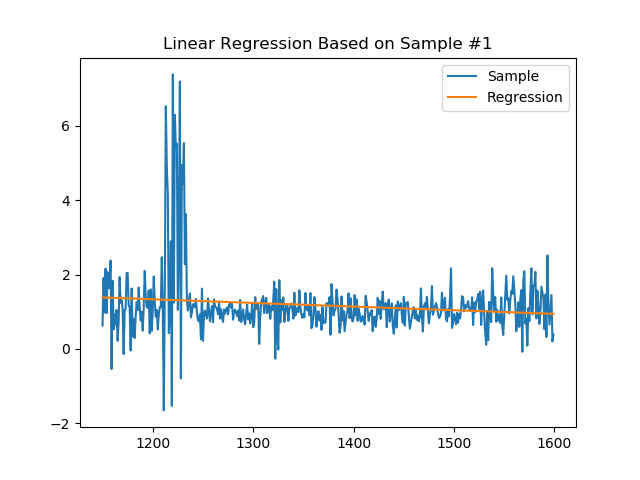
\includegraphics[width=0.80\textwidth]{figure/Regression4Quasar/b_i.png}
        \end{figure}
        \item
        Let $\theta = (X^TWX)^{-1}X^TW \vec{y}$, we can get the result
        \begin{figure}[H]
            \centering
            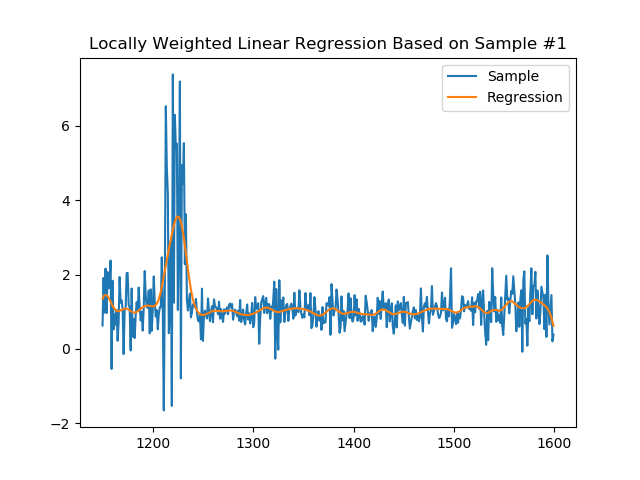
\includegraphics[width=0.60\textwidth]{figure/Regression4Quasar/b_ii.png}
        \end{figure}
        \item
        let $\tau$ be different value, we can get different fitting result.
        \begin{figure}[H]
            \centering
            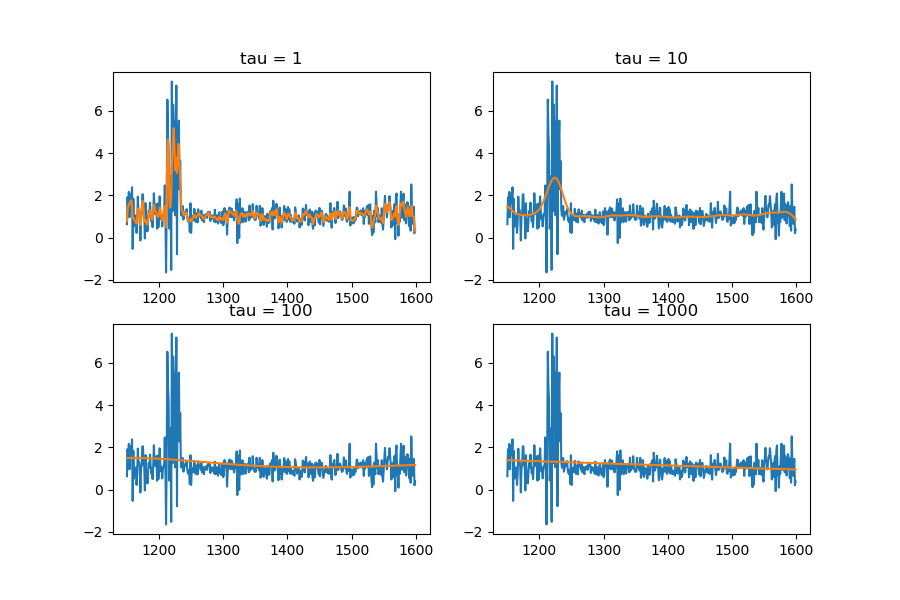
\includegraphics[width=0.80\textwidth]{figure/Regression4Quasar/b_iii.png}
        \end{figure}
        From the figure above, we know that, when $\tau = 1$, we get a perfect fitting result, but it's likely to be overfitting.\\
        As $\tau$ grows, the fitting gets worse and worse. So if we want to get a good result, we'd better trade off and select $\tau = 10$ (just an example) to get a balanced performance.

    \end{enumerate}
    \item
    \begin{enumerate}[label=(\roman*)]
        \item Just apply locally weighted linear regression to all 200 samples
        \item 
    
    \end{enumerate}

    \end{enumerate}  
\end{document}